\section{Data}

Data has become the foundation of decision-making, shaping industries and redefining business strategies. 
The journey of data-driven innovation can be divided into several key phases:

\begin{chronology}[5]{2010}{2025}{0.9\textwidth}
    \event[2012]{2015}{Big data}
    \event[2015]{2018}{Machine Learning}
    \event[2014]{2017}{Cloud computing}
    \event[2017]{2025}{Generative AI}
\end{chronology}

\paragraph*{Big data} 
Big data refers to the exponential growth of structured and unstructured data generated daily. 
It brought new challenges in storage, management, and analysis but also unlocked vast opportunities for business intelligence.
\renewcommand*{\arraystretch}{1.5}
\begin{table}[H]
    \centering
    \begin{tabular}{|l|l|}
    \hline
    \textbf{Technology} & Hadoop, Hive, Impala, Cloudera                                           \\ \hline
    \textbf{Key impact} & Data-driven decision-making, process optimization, competitive advantage \\ \hline
    \end{tabular}
\end{table}
\renewcommand*{\arraystretch}{1}

\paragraph*{Machine Learning}
Machine Learning marked the next stage of data evolution, enabling computers to learn patterns and make decisions without explicit programming. 
Machine Learning applications expanded rapidly, offering predictive insights and automation capabilities.
\renewcommand*{\arraystretch}{1.5}
\begin{table}[H]
    \centering
    \begin{tabular}{|l|l|}
    \hline
    \textbf{Technology} & Neural Networks, Deep Learning, Reinforcement Learning, Clustering                                  \\ \hline
    \textbf{Key impact} & Advanced automation, improved predictions, enhanced decision-making \\ \hline
    \end{tabular}
\end{table}
\renewcommand*{\arraystretch}{1}

\paragraph*{Cloud Computing}
Cloud computing revolutionized data storage and processing by providing scalable, cost-effective solutions over the internet. 
Businesses gained access to flexible computing power, reducing infrastructure constraints.
\renewcommand*{\arraystretch}{1.5}
\begin{table}[H]
    \centering
    \begin{tabular}{|l|l|}
    \hline
    \textbf{Technology} & AWS, Google Cloud Platform, Microsoft Azure                                 \\ \hline
    \textbf{Key impact} & Scalability, cost reduction, innovation acceleration \\ \hline
    \end{tabular}
\end{table}
\renewcommand*{\arraystretch}{1}

\paragraph*{Generative Artificial Inteligence}
Generative AI represents the latest frontier, where AI systems exhibit human-like understanding, learning, and application of knowledge across diverse domains.
Its potential is reshaping industries and redefining human-technology interaction.
\renewcommand*{\arraystretch}{1.5}
\begin{table}[H]
    \centering
    \begin{tabular}{|l|l|}
    \hline
    \textbf{Technology} & Large Language Models, synthetic data, Retrieval-Augmented Generation                                 \\ \hline
    \textbf{Key impact} & Creative automation, enhanced productivity, AI-driven decision making \\ \hline
    \end{tabular}
\end{table}
\renewcommand*{\arraystretch}{1}

\begin{figure}[H]
    \centering
    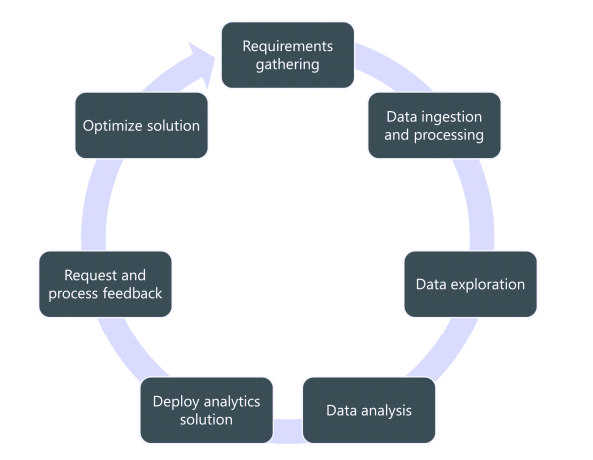
\includegraphics[width=0.5\linewidth]{images/bis10.png}
    \caption{Data framework}
\end{figure}


\subsection{Data job roles}

\paragraph*{Data and Cloud architect}
Data architects design comprehensive data infrastructures based on business objectives, ensuring seamless data integration and optimal storage solutions. 
Cloud Architects specialize in designing scalable, cloud-based architectures to support modern data needs.

\paragraph*{Data engineer}
Data engineers build and maintain the systems required for collecting, processing, and storing data. 
They design ETL pipelines, work with big data technologies, and ensure that raw data is transformed into a usable format.

\paragraph*{Data analyst}
Data analysts interpret and analyze data to provide actionable insights. 
They clean datasets, perform statistical analysis, and create visualizations to support business strategies and decision-making.

\paragraph*{Data scientist}
Data scientists develop machine learning models and apply advanced analytics to uncover patterns and predictions from complex datasets. 
They work with programming languages like Python and utilize AI-driven techniques for deeper insights.

\paragraph*{Data privacy and security specialist}
Data privacy officers ensure compliance with data protection regulations (e.g., GDPR), while security officers implement safeguards to protect organizational data from cyber threats and breaches.

\subsection{Data storage}
\begin{figure}[H]
    \centering
    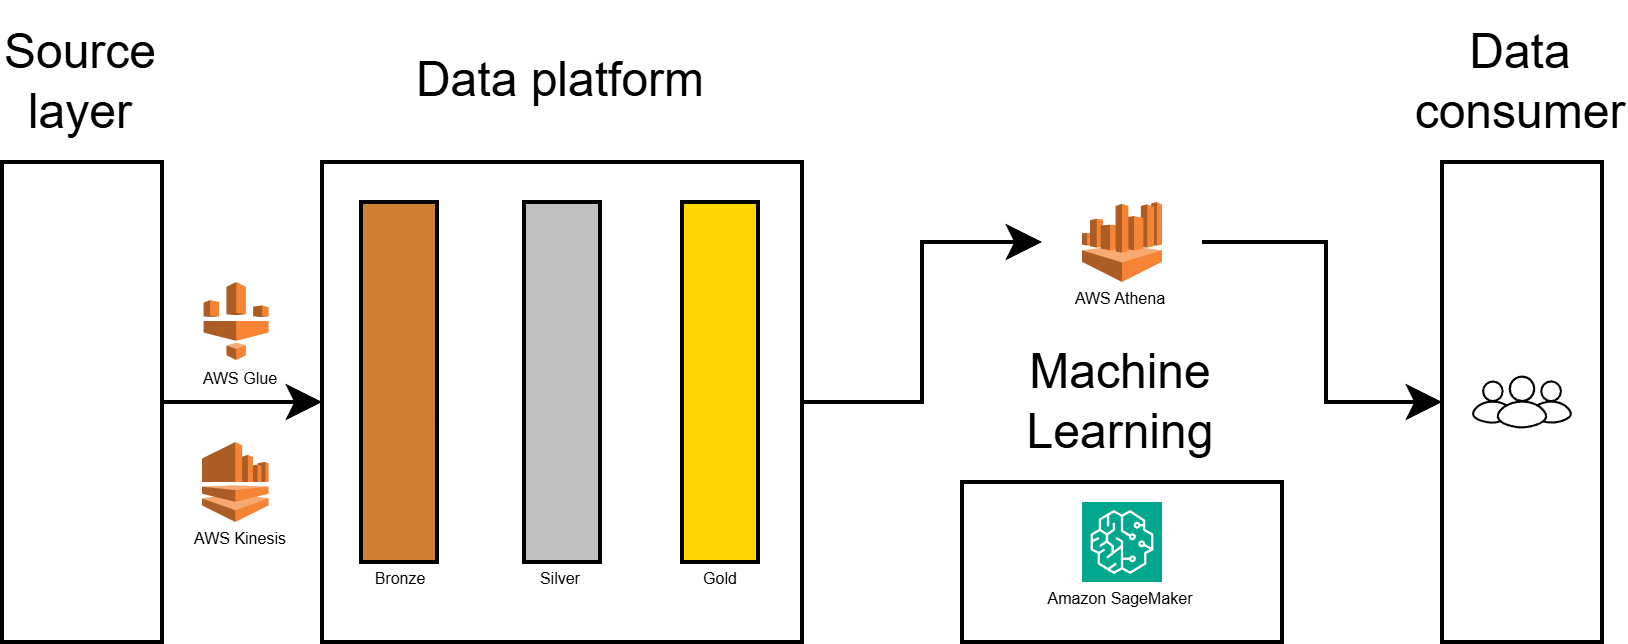
\includegraphics[width=0.75\linewidth]{images/bis11.png}
    \caption{Data architecture}
\end{figure}
The data architecture is structured as follows:
\begin{enumerate}
    \item \textit{Source layer}: this is where raw data originates, coming from operational systems, websites, e-commerce platforms, and other sources.
    \item \textit{Data ingestion}: as data is collected from the source, it undergoes transformations to make it usable within the data platform. 
        This step ensures that the data is properly formatted for analysis, enabling it to generate value for businesses.
    \item \textit{Data platform}: this is where the core data analysis happens. 
        Given the large volume of data, robust systems are needed to process it effectively. 
        The data refinement process follows a tiered approach:
        \begin{itemize}
            \item \textit{Bronze layer}: raw ingested data.
            \item \textit{Silver layer}: data undergoes Extract, Transform, Load processing.
            \item \textit{Gold layer}: fully analyzed and user-friendly data, optimized for reporting and decision-making.
        \end{itemize}
    \item \textit{Machine Learning} (optional): in this stage, advanced analytics and machine learning techniques extract valuable insights and patterns from the processed data.
    \item \textit{Data consumer}: the final processed data and insights are presented to end users or integrated into other applications, often in a visualization tool like Tableau.
\end{enumerate}
\begin{definition}[\textit{Data warehouse}]
    A data warehouse is a centralized repository that stores large volumes of structured data from various sources within an organization.
\end{definition}
\noindent Unlike transactional databases, which prioritize real-time operations, data warehouses are designed for analytical queries and historical data analysis. 
They facilitate reporting, business intelligence, and decision-making by providing a consolidated and structured view of organizational data.
\begin{definition}[\textit{Data lake}]
    A data lake is a scalable repository that allows organizations to store vast amounts of raw, structured, semi-structured, and unstructured data.
\end{definition}
\noindent Unlike a data warehouse, a data lake does not impose a schema on the data upon ingestion. 
Instead, it retains data in its original format until it is needed for processing or analysis.
While data lakes provide flexibility for advanced analytics and machine learning, they require careful governance and security measures to maintain data quality.

\paragraph*{Data lakehouse}
Organizations often integrate data warehouses and data lakes as part of a comprehensive data strategy, leveraging the strengths of both approaches:
\begin{itemize}
    \item \textit{Data integration}: raw data is ingested into the data lake, preserving its original format and serving as a staging area before further processing.
    \item \textit{Data transformation}: Extract, Transform, Load processes can take place in both the data lake and data warehouse. 
        Structured data required for immediate reporting is transformed and stored in the warehouse, while raw and unstructured data remains in the lake for exploratory analysis.
\end{itemize}
\begin{definition}[\textit{Data lakehouse}]
    A data lakehouse is a hybrid approach that combines data warehouses and data lakes.
\end{definition}
\noindent It provides a unified architecture that supports structured, semi-structured, and unstructured data, enabling both traditional business intelligence and modern machine learning workflows.
\begin{definition}[\textit{Polyglot persistence}]
    Polyglot persistence refers to the practice of using multiple types of data storage technologies and databases within a single system. 
\end{definition}
\noindent Instead of relying on a single storage solution, organizations select the best-suited technology for each specific data type and use case, optimizing performance and scalability across different applications.

\subsection{Data mesh}
\begin{definition}[\textit{Data mesh}]
    Data Mesh is a modern approach to analytical data architecture that treats data as a product.
\end{definition}
\noindent It is domain-driven, meaning that data ownership is distributed among teams that have the best understanding of their data and how it is used.

The key idea behind Data Mesh is that no one understands data better than its owner. 
Instead of relying on a centralized data team, Data Mesh distributes data responsibilities to domain-specific teams. 
Each domain aligns with a business function rather than specific applications or systems.
Each domain manages its own data pipelines within a shared infrastructure and provides access to domain-specific data and functionalities via APIs.

Data Mesh aims to improve the way organizations handle data by focusing on three key objectives:
\begin{itemize}
    \item \textit{Business enablement}: democratizing data with a self-service approach, reducing dependence on IT.
    \item \textit{Data management}: simplifying data processing, organization, and governance.
    \item \textit{Organizational efficiency}: facilitating seamless exchange of data products between producers and consumers.
\end{itemize}

\renewcommand{\arraystretch}{1.5}
\begin{table}[!ht]
    \centering

    \begin{tabular}{|l|p{4cm}|p{4cm}|p{4cm}|}
        \hline
        \textbf{Feature} & \textbf{Data warehouse} & \textbf{Data lake} & \textbf{Data mesh} \\ \hline
        \textit{Centralization} & Centralized & Centralized & Decentralized \\ \hline
        \textit{Data structure} & Structured & Unstructured & Both \\ \hline
        \textit{Use cases} & Reporting & Advanced analytics & Data product \\ \hline
        \textit{Integration} & Data lake & Data warehouse & Autonomous \\ \hline
        \textit{Flexibility} & No & No & Yes \\ \hline
    \end{tabular}
\end{table}
\renewcommand{\arraystretch}{1}

\subsection{Data governance}
Data governance is the framework that defines how an organization manages its data to ensure accuracy, security, and compliance. 
It encompasses processes, roles, policies, standards, and metrics to optimize data usage, enabling a company to become truly data-driven.
\begin{figure}[H]
    \centering
    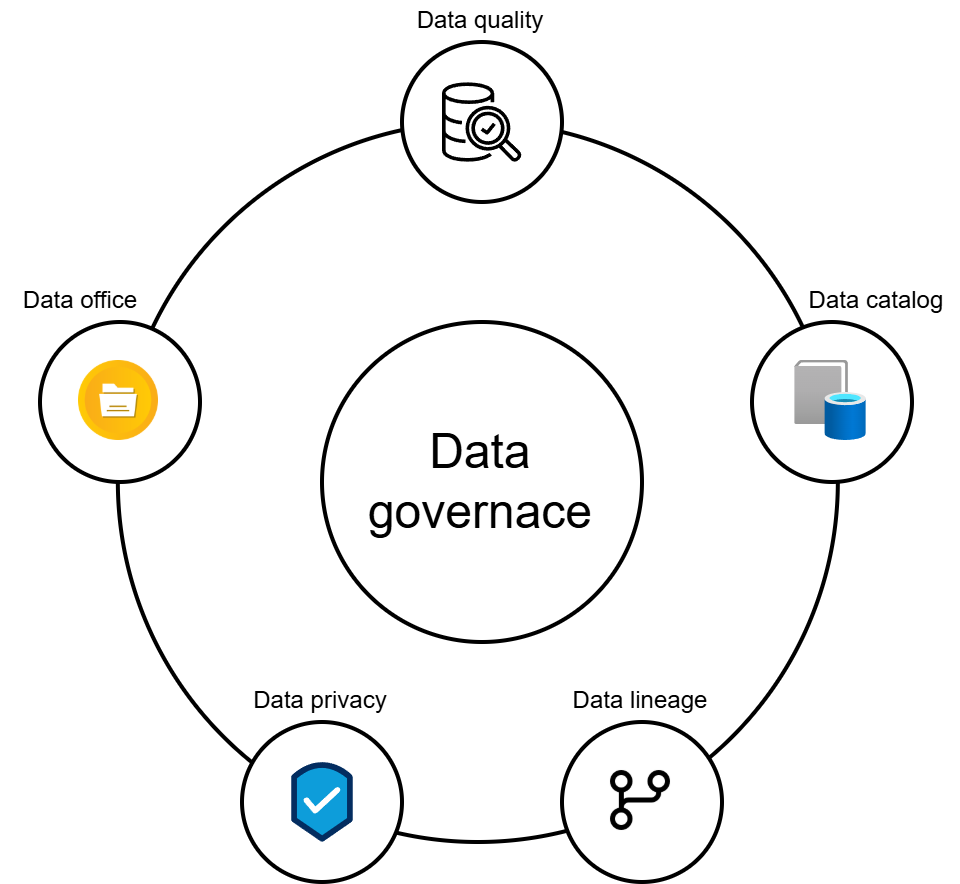
\includegraphics[width=0.5\linewidth]{images/bis12.png}
    \caption{Data governance pillars}
\end{figure}
Data governance relies on several foundational elements: 
\begin{itemize}
    \item \textit{Data quality}: ensures that information is accurate, reliable, and well-maintained. 
        It involves defining validation rules, monitoring quality at various stages, and using analytics to assess reliability. 
        AI-powered techniques, such as machine learning-driven validation, further enhance the integrity of data.
    \item \textit{Data catalog}: helps organizations manage and understand their data assets. 
        It integrates metadata from diverse sources such as databases, cloud platforms, ETL processes, and business intelligence tools. 
        By maintaining a structured data dictionary for IT teams and a data glossary for business users, companies can enhance collaboration and ensure consistency in data interpretation. 
        AI-driven search capabilities enable efficient metadata discovery and classification, supporting better knowledge sharing across the organization.
    \item \textit{Data lineage}: tracks the entire lifecycle of data, from its origin to its final destination. 
        By mapping transformations and interdependencies, it provides insights into how data moves through systems. 
        This capability is essential for assessing the impact of changes, optimizing service requests, and ensuring regulatory compliance. 
        Understanding data lineage also plays a crucial role in data protection, allowing organizations to pinpoint storage locations and enforce appropriate security measures.
    \item \textit{Data privacy}: focuses on the identification and safeguarding of sensitive information. 
        Effective privacy solutions assess risks, monitor data movement, and implement preventive measures to mitigate breaches. 
        Encryption, data masking, and access control policies ensure compliance with regulatory requirements while maintaining confidentiality. 
        Continuous analysis of data risks and proactive remediation strategies strengthen an organization's ability to protect its assets.
    \item \textit{Data office}: plays a key role in overseeing data governance initiatives. 
        Beyond technological solutions, governance efforts require clearly defined roles, responsibilities, and standardized management processes. 
        The Data Office establishes documentation templates, development guidelines, and monitoring frameworks to ensure governance policies are consistently applied.
\end{itemize}
\noindent Organizations rely on specialized technology platforms such as Informatica and Collibra to implement robust data governance strategies. 
These tools provide comprehensive capabilities for managing data quality, cataloging metadata, tracking lineage, and ensuring privacy. 
However, technology alone is not enough: effective governance requires a combination of tools, processes, and dedicated personnel within a structured Data Office.

Beyond compliance and data management, data governance serves as a strategic enabler for organizations. 
By establishing strong governance practices, companies can leverage their data assets more effectively, leading to innovations in areas such as data as a service and data monetization.

\paragraph*{Data monetization}
Data monetization transforms data into a valuable business asset by extracting insights that can be sold or leveraged for competitive advantage. 
High-quality, well-governed data enables businesses to identify new revenue opportunities, enhance market positioning, and strengthen partnerships.
With the right governance framework in place, organizations can shift from merely being data-driven to becoming proactive data providers, delivering insights that generate tangible business value.